
As the treatment effects reported in Section~\ref{sec:treatment-effects} show, there are gender differences in the patterns of positive and significant treatment effects. Similar gender differences have been seen in previous work. We summarize this previous work in Table~\ref{tab:litreview-table}. Our aggregating statistics and discussion of the counterfactual scenario allow for us to better summarize the gender differences and hint at mechanisms that can be driving these differences in treatment effects.

Figure~\ref{fig:ppositive} shows the estimated combining functions of the proportion of outcomes for which the estimated treatment effect is positive. As we explain in Section~\ref{sec:parameters}, the null hypothesis is that the proportion of outcomes is equal to 50\%. Figure~\ref{fig:ppositivehome} displays the combining functions comparing ABC/CARE to those who stay at home. Figure~\ref{fig:ppositivealternative} displays the same comparing ABC/CARE to those who attended alternative childcare. Both of these estimates account for selection into the counterfactual scenario using matching, as described in Section~\ref{sec:parameters}.

Comparing ABC/CARE to those who stay at home (Figure~\ref{fig:ppositivehome}), a higher proportion of the treatment effects are positive for women than for men. The female proportion is 25 percentage points larger than the male proportion. While the female proportion is significantly larger than 50\%, the standard error male proportion crosses the 50\%. We cannot reject the null hypothesis that ABC/CARE had more positive treatment effects for men relative to staying at home. 

Figure~\ref{fig:ppositivealternative} shows a different pattern comparing ABC/CARE to those who attended alternative childcare. Close to 75\% of the treatment effects are positive for men and we can reject the null hypothesis that ABC/CARE had more positive treatment effects for men relative to alternative childcare. For women, the proportion of positive treatment effects is similar to that comparing ABC/CARE to those who stay at home and is also statistically significantly different from 50\%. From these estimated combining functions, we can conclude that ABC/CARE was effective for men compared to alternative childcare, but not when compared to staying at home. ABC/CARE was effective for women regardless of the counterfactual scenario. 

\begin{figure}[!htbp]
\centering
\caption{Positively Impacted Outcomes, ABC/CARE Males and Females}\label{fig:ppositive}
\begin{subfigure}[h]{0.5\textwidth}
		\centering
		\caption{ Treatment vs.\ Stay at Home} \label{fig:ppositivehome}
		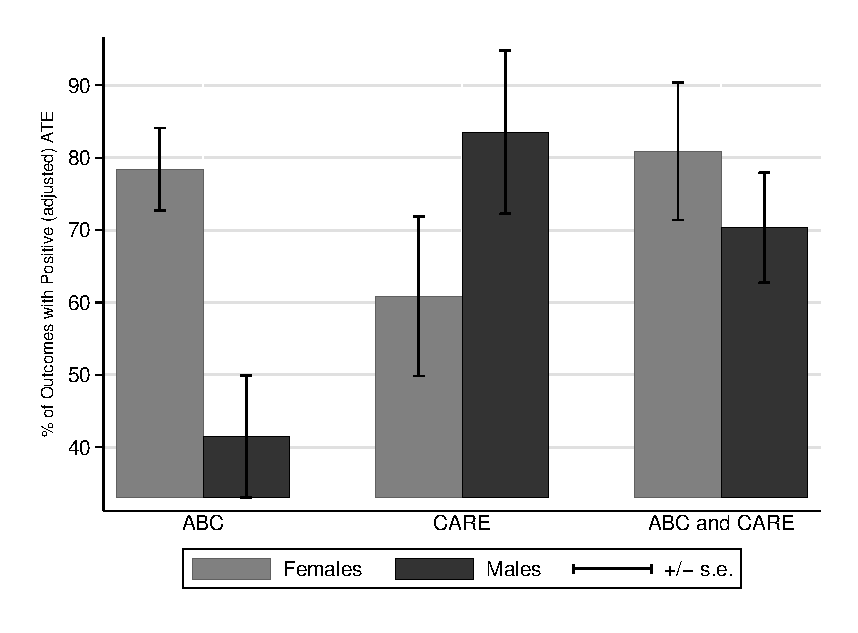
\includegraphics[width=\textwidth]{output/epan_ipw_p0_all.eps}
\end{subfigure}%
\begin{subfigure}[h]{0.5\textwidth}
	\centering
	\caption{Treatment vs.\ Alternative Childcare} \label{fig:ppositivealternative}
		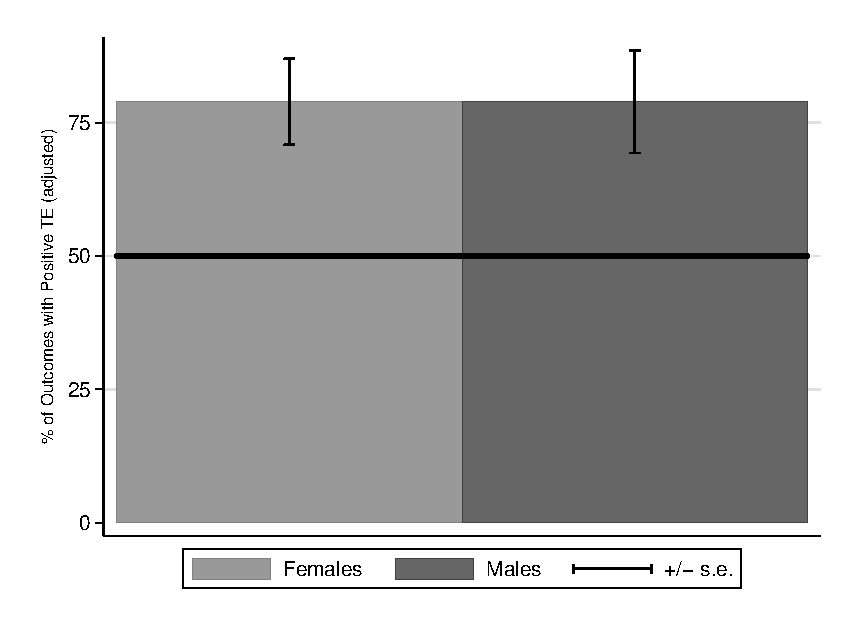
\includegraphics[width=\textwidth]{output/epan_ipw_p1_all.eps}
\end{subfigure}
\footnotesize \justify
\textbf{Note:} Panel (a) displays the percentage of positive treatment effects in accordance with the parameter in Equation~\eqref{eq:cont1}---treatment vs. staying at home---by gender. Panel (b) is analogous for Equation~\eqref{eq:cont2}---treatment vs.\ alternative childcare. Standard errors are based on the empirical bootstrap distribution. The null hypothesis is that the proportions of positive treatment effects are greater than 50\%. For a full list of the estimated combining functions, see Appendix~\ref{appendix:results}. \\
\end{figure}

We next show the estimated combining functions disaggregated by outcome category in Figure~\ref{fig:cats-positive}. Figure~\ref{fig:cats-positivehome} displays the proportions comparing ABC/CARE to staying at home and Figure~\ref{fig:cats-positivealt} displays the proportions comparing ABC/CARE to alternative childcare. Consistent with Figure~\ref{fig:ppositive} and the treatment effects reported in Section~\ref{sec:treatment-effects}, the female proportions are greater than or equal to the male proportions. The exception to this pattern is for eduction outcomes comparing ABC/CARE to staying at home in which the male proportion is larger than the female proportion, although the standard errors of the proportions overlap indicating that the difference between the two is not statistically significant. 

Comparing the male proportions across counterfactual scenarios, we find that ABC/CARE is more effective compared to alternative childcare than compared to staying at home. The exceptions to this pattern are seen in HOME scores and education. The opposite pattern is seen for women. The female proportions are larger comparing ABC/CARE to staying at home than comparing ABC/CARE to alternative childcare. Although in aggregating across all outcome categories, ABC/CARE seems equally effective for women by counterfactual scenario, disaggregating reveals that there are some outcome categories for which the proportions comparing ABC/CARE to staying at home are larger than comparing ABC/CARE to alternative childcare. These categories include HOME scores, mental health, employment and income, and crime. These results indicate that ABC/CARE is more effective for women when compared to staying at home and more effective for men when compared to alternative childcare.


\begin{figure}[H]
 \centering
 \caption{Proportion of Positively Impacted Outcomes by Category}\label{fig:cats-positive}
 \begin{subfigure}[h]{0.7\textwidth}
 	\centering
 	\caption{Treatment vs.\ Stay at Home} \label{fig:cats-positivehome}
 		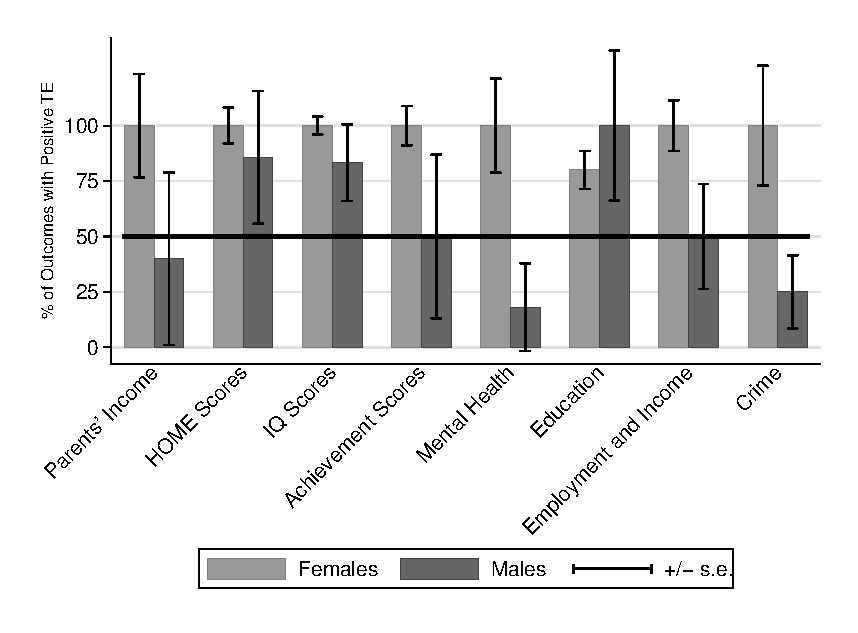
\includegraphics[width=\textwidth]{output/epan_ipw_p0_cats1.eps}
 \end{subfigure}
 
 \begin{subfigure}[h]{0.7\textwidth}
 	\centering
 	\caption{Treatment vs.\ Alternative Childcare} \label{fig:cats-positivealt}
 		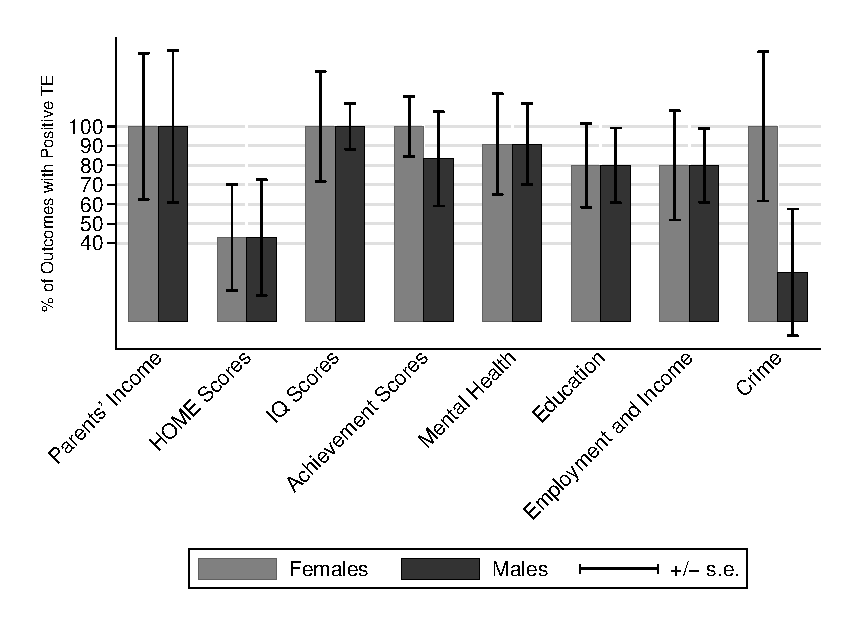
\includegraphics[width=\textwidth]{output/epan_ipw_p1_cats1.eps}
 \end{subfigure}
 \footnotesize \justify
\footnotesize \justify
\textbf{Note:} Panel (a) displays the percentage of positive treatment effects by outcome category in accordance with the parameter in Equation~\eqref{eq:cont1}---treatment vs. staying at home---by gender. Panel (b) is analogous for Equation~\eqref{eq:cont2}---treatment vs.\ alternative childcare. Standard errors are based on the empirical bootstrap distribution. The null hypothesis is that the proportions of positive treatment effects are greater than 50\%. For a full list of the estimated combining functions, see Appendix~\ref{appendix:results}. \\
 \end{figure}

\begin{sidewaysfigure}[!htpb]
\centering
\caption{Gender and Baseline Socioeconomic Disadvantage in the Control Group} \label{figure:socdis}
\begin{subfigure}[h]{0.4\textwidth}
	\centering
	\caption{Take-up of Alternatives by Gender} \label{figure:altgender}
	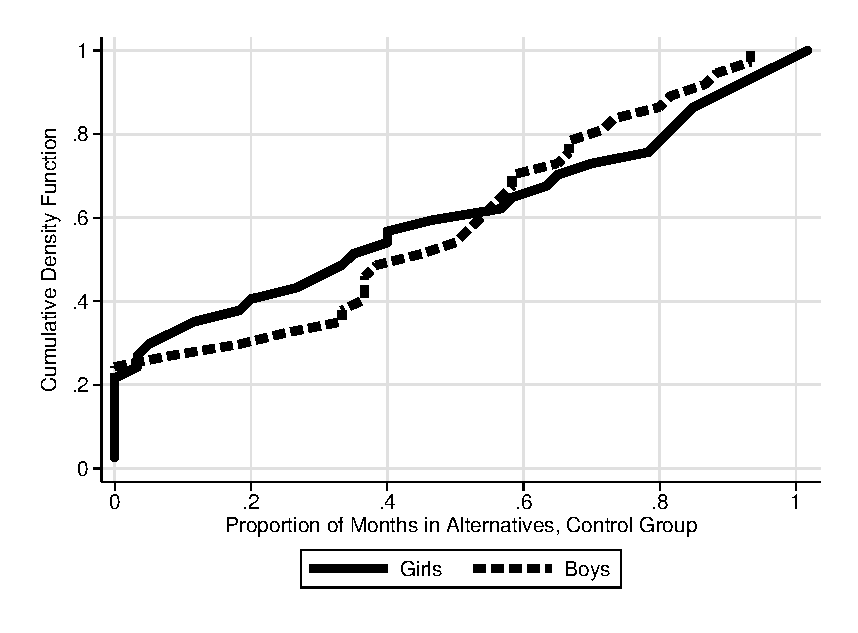
\includegraphics[width=\textwidth]{output/abccare_controlcontamination_boysgirls}
\end{subfigure}%
\begin{subfigure}[h]{0.4\textwidth}
	\centering
	\caption{Socioeconomic Disadvantage by Gender} \label{figure:disadgender}
	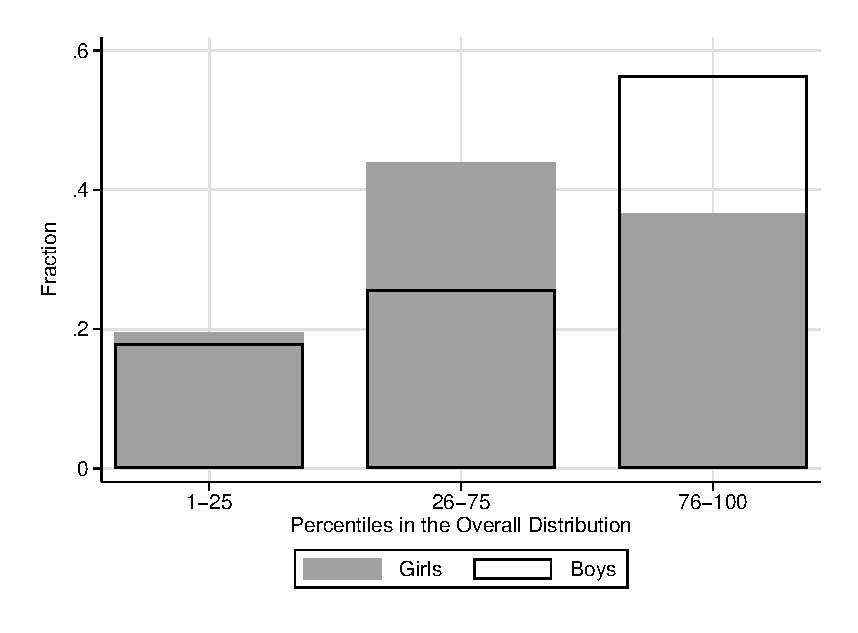
\includegraphics[width=\textwidth]{output/factorbase_girlsboyscompare}
\end{subfigure}
\begin{subfigure}[h]{0.4\textwidth}
	\centering
	\caption{Disadvantage by Take-up of Alternatives, Girls} \label{figure:disadgirls}
	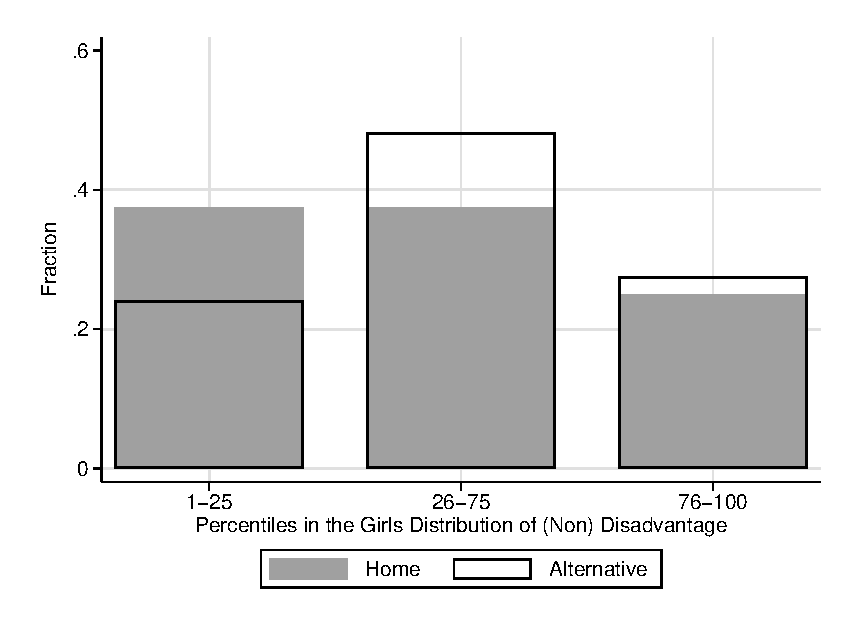
\includegraphics[width=\textwidth]{output/factorbase_wgirlscompare}
\end{subfigure}%
\begin{subfigure}[h]{0.4\textwidth}
	\centering
	\caption{Disadvantage by Take-up of Alternatives, Boys} \label{figure:disadboys}
	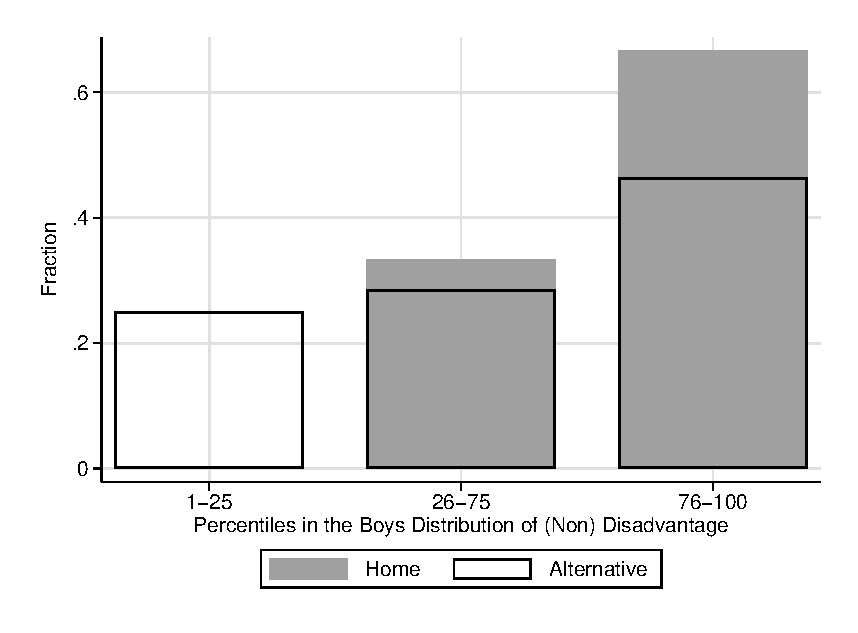
\includegraphics[width=\textwidth]{output/factorbase_wboyscompare}
\end{subfigure}
\footnotesize
\justify
\textbf{Note:} Panel (a) displays the cumulative distribution function of enrollment in alternatives by gender. Panel (b) displays how girls and boys separately fit into the overall (girls and boys pooled) distribution of socioeconomic disadvantage. Panel (c) displays how girls who did not enroll and girls who enrolled in alternatives fit into the overall female distribution of socioeconomic disadvantage. Panel (d) is analogous to Panel (c) for boys. Our measure of socioeconomic disadvantage is a latent of the following variables: Maternal age, education, and IQ, as well as number of siblings and HRI score.
\end{sidewaysfigure}

This difference suggests that boys and girls faced different situations in their counterfactual environments, especially in the home environments. Table~\ref{table:controlsubscharacteristics} summarizes the baseline characteristics by gender and counterfactual scenario. Approximately the same proportion of control-group girls attended alternative childcare (73\%)  as control-group boys (76\%). We confirm that the take-up of amount alternative childcare is similar across genders in Figure~\ref{figure:altgender}. 

Maternal employment of mothers of girls is the only statistically significant difference between those who stayed at home and those who attended alternative childcare. No girls who stayed at home had working mothers while 23\% of the girls who attended alternative childcare had working mothers. For boys, 14\% of those who stayed at home had working mothers while 29\% of those who attended alternative childcares had working mothers. As we show in Section~\ref{sec:treatment-effects}, ABC/CARE increases maternal income. It is also clear that control-group children who attend alternative childcare are more likely to have working mothers. Pooling genders, 26\% of those who attended alternative childcare had working mothers versus 8\% of those who stayed at home. Although the alternative childcares were not substitutes for ABC/CARE in terms of quality, educational offerings, or child outcomes, they did provide between 3 and 8 hours of childcare per day to allow the mothers to work (or continue working).

\begin{sidewaystable}[H]
\centering
\begin{threeparttable}
\caption{Baseline Characteristics and Control Substitution}\label{table:controlsubscharacteristics}
\begin{tabular}{l c c}
\toprule
Characteristic & \mc{2}{c}{Control Substitution} \\
& No & Yes \\
& $ N=19 $ & $ N=55 $ \\
\midrule
Mother's Yrs. of Edu. &      9.74 &     10.35 \\
                     & (     0.43) & (     0.26)  \\
Mother's Age &     21.42 &     20.27 \\
                     & (     1.79) & (     0.63)  \\
Mother's IQ &     82.00 &     85.60 \\
                     & (     2.32) & (     1.33)  \\
HRI Score &     20.95 &     21.60 \\
                     & (     1.46) & (     0.81)  \\
Number of Siblings &      1.00 &      0.62 \\
                     & (     0.38) & (     0.13)  \\
Male &      0.47 &      0.51 \\
                     & (     0.12) & (     0.07)  \\
Birth Year &   1975.58 &   1975.73 \\
                     & (     0.68) & (     0.32)  \\
Apgar Score, 1 min. &      7.47 &      7.62 \\
                     & (     0.43) & (     0.21)  \\
Apgar Score, 5 min. &      8.63 &      8.98 \\
                     & (     0.26) & (     0.14)  \\
\bottomrule
\end{tabular}
\begin{tablenotes}
\item \footnotesize \textbf{Note:} This table describes baseline characteristics for the children in the control group, by gender and by their enrollment in alternative childcare. The number of subjects in these groups are listed at the top of the table. Asymptotic standard errors are in parentheses. The reported $p$-values are from two-sided tests of difference of means. The means are bolded if the difference is significant at the 10\% level. In Table~\ref{tab:abccare-baseline}, we jointly test for baseline differences between males and females and between treatment- and control-group children, accounting for multiple hypotheses, and find that none of the $p$-values remain significant after this adjustment.
\end{tablenotes}
\end{threeparttable}
\end{sidewaystable}

The difference in maternal labor supply indicates that there is some special difference in the family characteristics of control-group boys who stayed at home relative to control-group boys who attended alternative care and control-group girls. The control-group boys who stayed at home also have older mothers, more fathers present, lower HRI scores, and more siblings than any of the other subgroups. Of course, these characteristics are interrelated. For example, having a father at home implies that the family income is higher. This is due to the father brining additional income rather than the presence of the father allowing the mother to work, given that the association between father's presence and maternal employment is weak. 

To formally test the differences in control-group girls and boys, we create a latent measure of socioeconomic disadvantage at baseline using the following variables: Mother's age, education, IQ, marital status, and employment, as well as number of children and father's presence at home. We assess how girls and boys fit into the overall distribution of this latent in the control group. Boys are disproportionately more advantaged than girls (Panel~\ref{figure:disadgender}). Because girls' families were more resource constrained if compared to their male counterparts, girls in the control group were taken care of in a more disadvantaged environment or went to lower-quality preschools. Thus, they benefited more than boys when compared to the next best alternative as perceived by their parents, as documented in Section~\ref{sec:treatment-effects}.

Table~\ref{table:disadtests} uses the latent measure to test the difference in disadvantage across boys and girls. We reject the null of a common distribution of our measure of socioeconomic disadvantage across girls and boys (at baseline). In Panels~\ref{figure:disadgirls} and~\ref{figure:disadboys} of Figure~\ref{figure:socdis}, we further dissect socioeconomic disadvantage within genders, and provide the corresponding tests in Table~\ref{table:disadtests}.

\begin{table}[!htpb]
\begin{threeparttable}
\caption{Gender and Baseline Socioeconomic Disadvantage in the Control Group, Tests} \label{table:disadtests}
\centering
\begin{tabularx}{16.5cm}{XcX}
& \begin{tabular}{cccc}
\toprule
Males vs. Females & & \mc{2}{c}{Alt. vs. Home} \\
\cmidrule(lr){1-2} \cmidrule(lr){3-4}
Control Group & & Males & Females \\
\midrule
\textbf{0.007} & & \textbf{0.006} & 0.110 \\
\bottomrule
\end{tabular}

% Control, males vs. females: distance between: factor of m_age_base, m_ed_base, m_iq_base, hh_sibs_base, hrabc_index

% Alt. vs home: factor of m_age_base, m_ed_base, m_iq_base, hh_sibs_base, hrabc_index &
\end{tabularx}
\begin{tablenotes}
\footnotesize
\item \textbf{Note:} This table presents the null of a distribution of the latent measure of socioeconomic disadvantage (mother's age, education, IQ, marital status, and employment, as well as number of siblings and father's presence at home) between males and females in the control group and between children who attended  alternative preschool and who stayed at home (within control-group boys or within control-group girls). The $p$-values follow \citet{Rosenbaum_2005_Distribution_JRSS}. Under the null hypothesis, the pairs with the closest distance in disadvantage would be comprised of one male and one female (for the comparison of males vs. females). Rejecting the null implies that the distributions are significantly different. Statistics significant at the $0.10$ level are bolded.
\end{tablenotes}
\end{threeparttable}
\end{table}

Parents of more advantaged girls are more likely to send their daughters to alternative preschools. Parents of more advantaged boys are more likely to keep their sons at home. Thus, boys benefited more from treatment when compared to attending alternative childcare as opposed to staying at home where they faced a better environment. The opposite pattern holds for girls, although the differences between the estimates by counterfactual scenario are smaller for girls than for boys. This is consistent with Table~\ref{table:disadtests}, which shows that while the selection into alternative childcare statistically significantly differs by family disadvantage for boys, it is not statistically significant for girls. 
